\pdfoutput=1
\documentclass[12pt]{article}
\usepackage{amsmath, amssymb, amsthm}
\usepackage{graphicx}
\graphicspath{{../}}
\usepackage{booktabs}
\usepackage{array}
\usepackage[colorlinks=true, linkcolor=blue, citecolor=blue, urlcolor=blue]{hyperref}
\usepackage[numbers,sort&compress]{natbib}
\usepackage{listings}
\usepackage{xcolor}
\lstset{language=Python,basicstyle=\ttfamily\footnotesize,
  keywordstyle=\color{blue!80!black},commentstyle=\color{gray},
  stringstyle=\color{orange!80!black},showstringspaces=false,breaklines=true,
  frame=single,numbers=left,numberstyle=\tiny\color{gray},captionpos=b}
\newtheorem{theorem}{Theorem}[section]
\newtheorem{lemma}[theorem]{Lemma}
\newtheorem{proposition}[theorem]{Proposition}
\newtheorem{corollary}[theorem]{Corollary}
\newtheorem{conjecture}[theorem]{Conjecture}
\theoremstyle{definition}
\newtheorem{definition}[theorem]{Definition}
\theoremstyle{remark}
\newtheorem{remark}[theorem]{Remark}
\title{Emergence of Classical Constants from a Minimal Recursive Triadic Framework}
\author{J. W. Milton\\[4pt]\small Clarity Coalition}
\date{10 June 2026 \\ \small v1.2}
\begin{document}
\maketitle

\begin{abstract}
Five classical mathematical constants (the Leibniz limit $\pi/4$, the golden ratio
$\varphi$, Euler's number $e$, $\sqrt{2}$, and $\ln 2$) emerge as limits of a single
family of three-variable recurrences on a triple $(N, D, C)$ with functionally distinct
roles: a \emph{negotiation} state that is iteratively refined, a
\emph{definition\,/\,limitation} parameter that bounds, and a
\emph{contribution\,/\,integration} parameter that accumulates. These roles are
irreducible to fewer than three even when two positions share the same numerical seed value.

Each branch is specified by an initial triple $(N_0, D_0, C_0)$ and a \emph{traversal rule}
governing the evolution of $(D_k, C_k)$. The five branches fall into three traversal classes:
Advancing (Class~A, external parameter injection), Self-redefined (Class~B, internal
transformation), and Fixed (Class~C, constant parameters). The limits are classical: each
branch reduces to a known series, fixed point, or iterative method, so the contribution of
this framework is not in computing these numbers anew, but in \emph{structural unification}:
a single three-role grammar from which all five mechanisms descend, combined with proved
theorems (diagonal invariance, swap symmetry, perfect-square denominators, offset
consistency, parametric families).
  
The $\pi/4$ branch is structurally unique: it alone requires three numerically distinct seeds
$\{1, 3, 5\}$ and advances its parameters externally via a fixed step $\Delta = 4$ rooted in
a geometric axis structure. The remaining four branches operate on seeds from $\{0, 1, 2\}$
with purely internal or fixed parameter evolution. Four open conjectures address whether these
assignments are forced by the framework or merely convenient choices.
\end{abstract}

\noindent\textbf{MSC 2020:} 40A05 (primary); 11B39, 65B10 (secondary).

\noindent\textbf{Keywords:} classical constants; recursive sequences; triadic recurrence;
Fibonacci ratio; alternating series; structural unification.

\tableofcontents
\section{Introduction}\label{sec:intro}

The Leibniz series for $\pi/4$,
\[
  \frac{\pi}{4} = 1 - \frac{1}{3} + \frac{1}{5} - \cdots
  = \sum_{k=0}^{\infty} \frac{(-1)^k}{2k+1},
\]
has been known since the late seventeenth century and remains a landmark example of
slowly convergent alternating series \cite{Lei82,Roy11}. Leibniz himself saw
philosophical significance in binary arithmetic and its connection to the I~Ching
\cite{Lei03}, viewing the interplay of 0 and~1 as a model of structured emergence from
minimal premises.

Five real numbers recur persistently across mathematics: $\pi$, the golden ratio
$\varphi = (1+\sqrt{5})/2$, Euler's number $e$, $\sqrt{2}$, and $\ln 2$. Each has
multiple independent characterizations and has been analyzed in isolation over centuries.
The question of whether a \emph{single algebraic apparatus} organizes all five as
co-equal outputs of one recursive scheme is less a question of computing them anew than
one of \emph{structural unification}: does a common grammar exist?

This paper answers that question affirmatively for the \emph{tholonic ladder}: a family
of three-variable recurrences whose branches are distinguished by different initial
triples and traversal rules, but whose variable roles remain consistent across all five instances.

\textbf{What this paper provides.} Minimal definitions; a complete branch-specification
table; full proofs of convergence to each classical limit; structural theorems with proofs;
quantitative convergence data; and four open conjectures.

\textbf{What this paper does not provide.} New proofs of the underlying series
identities: those are classical and referenced. The contribution is the shared grammar
and the structural contrasts.

\textbf{Organization.}
\S\,\ref{sec:triad} defines the tholonic triad and motivates its geometry.
\S\,\ref{sec:irreducible} argues the irreducibility of three variables.
\S\,\ref{sec:ladder} introduces the ladder family and its traversal-class taxonomy.
\S\,\ref{sec:branches} provides the complete branch specification and proves the five
convergence propositions.
\S\,\ref{sec:structural} establishes the structural properties.
\S\,\ref{sec:convergence} records convergence data.
\S\,\ref{sec:open} states four open conjectures.
\S\,\ref{sec:related} covers related work.
\S\,\ref{sec:discussion} discusses scope and implications.
\S\,\ref{sec:conclusion} concludes.

\section{The tholonic triad}\label{sec:triad}

\begin{definition}[Tholonic triad]\label{def:triad}
A \emph{tholonic triad} is an ordered triple $(N, D, C)$ of non-negative reals together
with three directed relational roles:
\begin{itemize}
  \item $N$ (\emph{negotiation}): the running state; the quantity being iteratively
        refined, emerging from the interaction of the other two.
  \item $D$ (\emph{definition\,/\,limitation}): the constraining, bounding force; what
        \emph{limits} the state.
  \item $C$ (\emph{contribution\,/\,integration}): the accumulating, synthesizing force;
        what \emph{grows} the state.
\end{itemize}
The triad is not merely a vector: the three positions have distinct semantic roles that
persist across all five branches, regardless of whether two positions share a numerical value.
\end{definition}

\subsection{Geometric origin of the axis labels}\label{subsec:geometry}

The tholonic geometry \cite{Mil24} assigns successive powers of two, $2^0, 2^1, \ldots, 2^5$,
to six vertices of a triangular configuration: outer role vertices $N = 2^0$, $D = 2^1$,
$C = 2^2$, and three inner midpoint vertices carrying $2^3, 2^4, 2^5$. Each directed axis
runs from one outer role vertex through an inner midpoint to another outer role vertex;
its three vertex values sum to $7$ times a characteristic multiplier:
\begin{itemize}
  \item Definition axis ($N \to D$, through $2^5$):\quad $1 + 32 + 2 = 35 = 7 \times 5$
  \item Contribution axis ($C \to N$, through $2^4$):\quad $4 + 16 + 1 = 21 = 7 \times 3$
  \item Instantiation axis ($D \to C$, through $2^3$):\quad $2 + 8 + 4 = 14 = 7 \times 2$
\end{itemize}
The Instantiation axis multiplier, denoted $\mathrm{istep} = 2$, enters the $\pi/4$ branch:
\[
  d_{\mathrm{step}} = \mathrm{istep}^2 = 4,\qquad c_{\mathrm{step}} = 2 \times \mathrm{istep} = 4.
\]
Both equal~$4$, fixing step size $\Delta = 4$ without free parameters. The seed triple
$(N_0, D_0, C_0) = (1, 3, 5)$ receives a geometric interpretation. Each axis connects two
of the three roles and excludes the third, and its multiplier supplies the seed (or step)
of precisely the excluded role: the Definition axis ($N \to D$) excludes $C$ and carries
$5 = C_0$; the Contribution axis ($C \to N$) excludes $D$ and carries $3 = D_0$; the
Instantiation axis ($D \to C$) excludes $N$ and carries $\mathrm{istep} = 2$, which fixes
$\Delta = 4$ above. The seeds $3$ and~$5$ are simultaneously the first members of the
$(4n-1, 4n+1)$ parity classes traversed by the recursion, and $N_0 = 1$ is the
multiplicative identity. Each role draws its seed from the complementary axis, so the
axis geometry supplies both the seeds and the step that drives them.
This motivates the seed-partition theorem of Proposition~\ref{prop:seed-partition}.

\begin{figure}[ht]
  \centering
  \includegraphics[width=\linewidth,keepaspectratio]{figures/1_tholonic-triad}
  \caption{Left: the tholonic triad. Outer vertices carry roles $N$, $D$, $C$ with
    values $2^0, 2^1, 2^2$; inner midpoint vertices carry $2^3, 2^4, 2^5$. Each
    directed axis sums to a multiple of~$7$ (multipliers $5$, $3$, $2$). Right: the
    Instantiation axis multiplier $\mathrm{istep}=2$ uniquely fixes $\Delta=4$ and
    the seed triple $(N_0, D_0, C_0) = (1, 3, 5)$.}
  \label{fig:tholonic-triad}
\end{figure}

\section{The irreducible three-variable structure}\label{sec:irreducible}

\begin{lemma}[Triadic irreducibility]\label{lem:irreducibility}
Let $\mathcal{R}$ be a recurrence on $m$ real variables $x^{(1)}, \ldots, x^{(m)}$ in which
the update to one distinguished state variable $x^{(1)}$ is of the form
\[
  x^{(1)}_{k+1} = g\!\left(x^{(1)}_k;\, \alpha_k,\, \beta_k\right),
\]
where $\alpha_k$ limits the correction magnitude and $\beta_k$ controls the additive or
multiplicative integration of each step. Suppose that \emph{(i)}~$\alpha_k$ and $\beta_k$
are functionally independent in the sense that $g$ is not expressible as a function of a
single combined argument $h(\alpha_k, \beta_k)$, and \emph{(ii)}~the limit
$L = \lim_{k\to\infty} x^{(1)}_k$ is not a trivial fixed point of a one- or two-variable
recurrence. Then $\mathcal{R}$ requires $m \geq 3$.
\end{lemma}
\begin{proof}
The distinguished variable $x^{(1)}$ must persist across iterations to record the refined
state, so it cannot be eliminated. Suppose $m = 2$. Then both control arguments are
determined by the single auxiliary variable $y_k$: $\alpha_k = a(y_k)$ and
$\beta_k = b(y_k)$, and the admissible pairs $(\alpha_k, \beta_k)$ are confined to the
one-parameter image of $y \mapsto (a(y), b(y))$. On that set, $g$ factors through the
single argument $y$ itself: $g(x;\, \alpha_k, \beta_k) = \tilde{g}(x;\, y_k)$, exhibiting
exactly the combined-argument factorization that hypothesis~\emph{(i)} excludes on the
admissible set. Hypothesis~\emph{(ii)} rules out the degenerate alternative in which the
controls are constant or absent and $L$ is reachable with fewer variables. Hence two
functionally independent auxiliary variables are required, and with the state variable,
$m \geq 3$.
\end{proof}

A critical structural property is that \textbf{every branch requires exactly three
variables}, regardless of whether some share the same numerical value.

In the $e$ branch, $D_0 = C_0 = 1$; in the $\sqrt{2}$ branch, $D_0 = C_0 = 2$. However,
the triad is not about three \emph{numbers}; it is about three \emph{functional roles}:
\begin{enumerate}
  \item \textbf{$N$}: the state being negotiated; what emerges.
  \item \textbf{$D$}: the defining boundary; what constrains.
  \item \textbf{$C$}: the integrating accumulator; what synthesizes.
\end{enumerate}
In the $e$ branch, $D = 1$ is the fixed numerator that never changes; the unchanging
boundary. $C$ starts at~$1$ but grows as a factorial. They begin at the same value but
diverge immediately in behavior: one constrains, the other integrates.

In the $\sqrt{2}$ branch, $D = 2$ is the target being bounded toward; the defining
constraint. $C = 2$ is the averaging divisor; the integrator that synthesizes overshoot
and undershoot. Without $D/N$, there is no correction; without $C$-division, no synthesis.

\textbf{The triad is irreducible: a state, a limiter, and a contributor constitute the
minimum structure for a recursion that converges to a non-trivial constant.}

\section{The ladder family}\label{sec:ladder}

\begin{definition}[Tholonic ladder recurrence]\label{def:ladder}
Given $(N_0, D_0, C_0) \in \mathbb{R}^3$, a \emph{tholonic ladder branch} is a discrete
dynamical system
\[
  N_{k+1} = f(N_k;\, D_k,\, C_k), \qquad k \in \mathbb{N}_0,
\]
together with a \emph{traversal rule} specifying how $(D_k, C_k)$ is updated at each step.
\end{definition}

\begin{definition}[Branch]\label{def:branch}
A \emph{branch} is the tuple $\bigl((N_0, D_0, C_0),\, f,\, \text{traversal rule}\bigr)$.
\end{definition}

\subsection{Classification of traversal types}\label{subsec:traversal}

\textbf{Class~A: Advancing.} $(D_k, C_k)$ each receive a fixed external increment at every
step. New information is injected per iteration. Only the $\pi/4$ branch belongs to this class.

\textbf{Class~B: Self-redefined.} $(D_k, C_k)$ evolve by a transformation of their own
current values (Fibonacci swap for $\varphi$, factorial scaling for $e$) with no external
increment. The factorial rule consumes the iteration counter $k$ as a multiplier, but
injects no new constant beyond it.

\textbf{Class~C: Fixed.} $(D_k, C_k)$ are held constant at their seed values for all $k$.
Convergence is driven by the update map $f$ alone: as a pure fixed-point iteration in the
$\sqrt{2}$ branch (where $k$ never enters $f$), or with the iteration index entering $f$
directly in the $\ln 2$ branch.

This trichotomy partitions the five branches cleanly: one Class~A ($\pi/4$), two Class~B
($\varphi$, $e$), two Class~C ($\sqrt{2}$, $\ln 2$). The classification can equivalently
be stated on two independent axes: whether $(D_k, C_k)$ evolve at all, and whether the
branch consumes the iteration counter $k$.
\begin{table}[ht]
\centering\caption{Two-axis refinement of the traversal classification.}\label{tab:two-axis}
\begin{tabular}{llll}\toprule
Branch & $(D, C)$ evolve? & Counter $k$ consumed? & Class \\\midrule
$\pi/4$    & yes (external increment $\Delta$) & no                & A \\
$\varphi$  & yes (internal swap)               & no                & B \\
$e$        & yes (scaling by $k$)              & yes, in traversal & B \\
$\sqrt{2}$ & no                                & no                & C \\
$\ln 2$    & no                                & yes, in $f$       & C \\\bottomrule
\end{tabular}\end{table}
Class~A is evolution by external constant; Class~B is evolution by internal or
counter-indexed transformation; Class~C is no evolution.

\begin{figure}[ht]
  \centering
  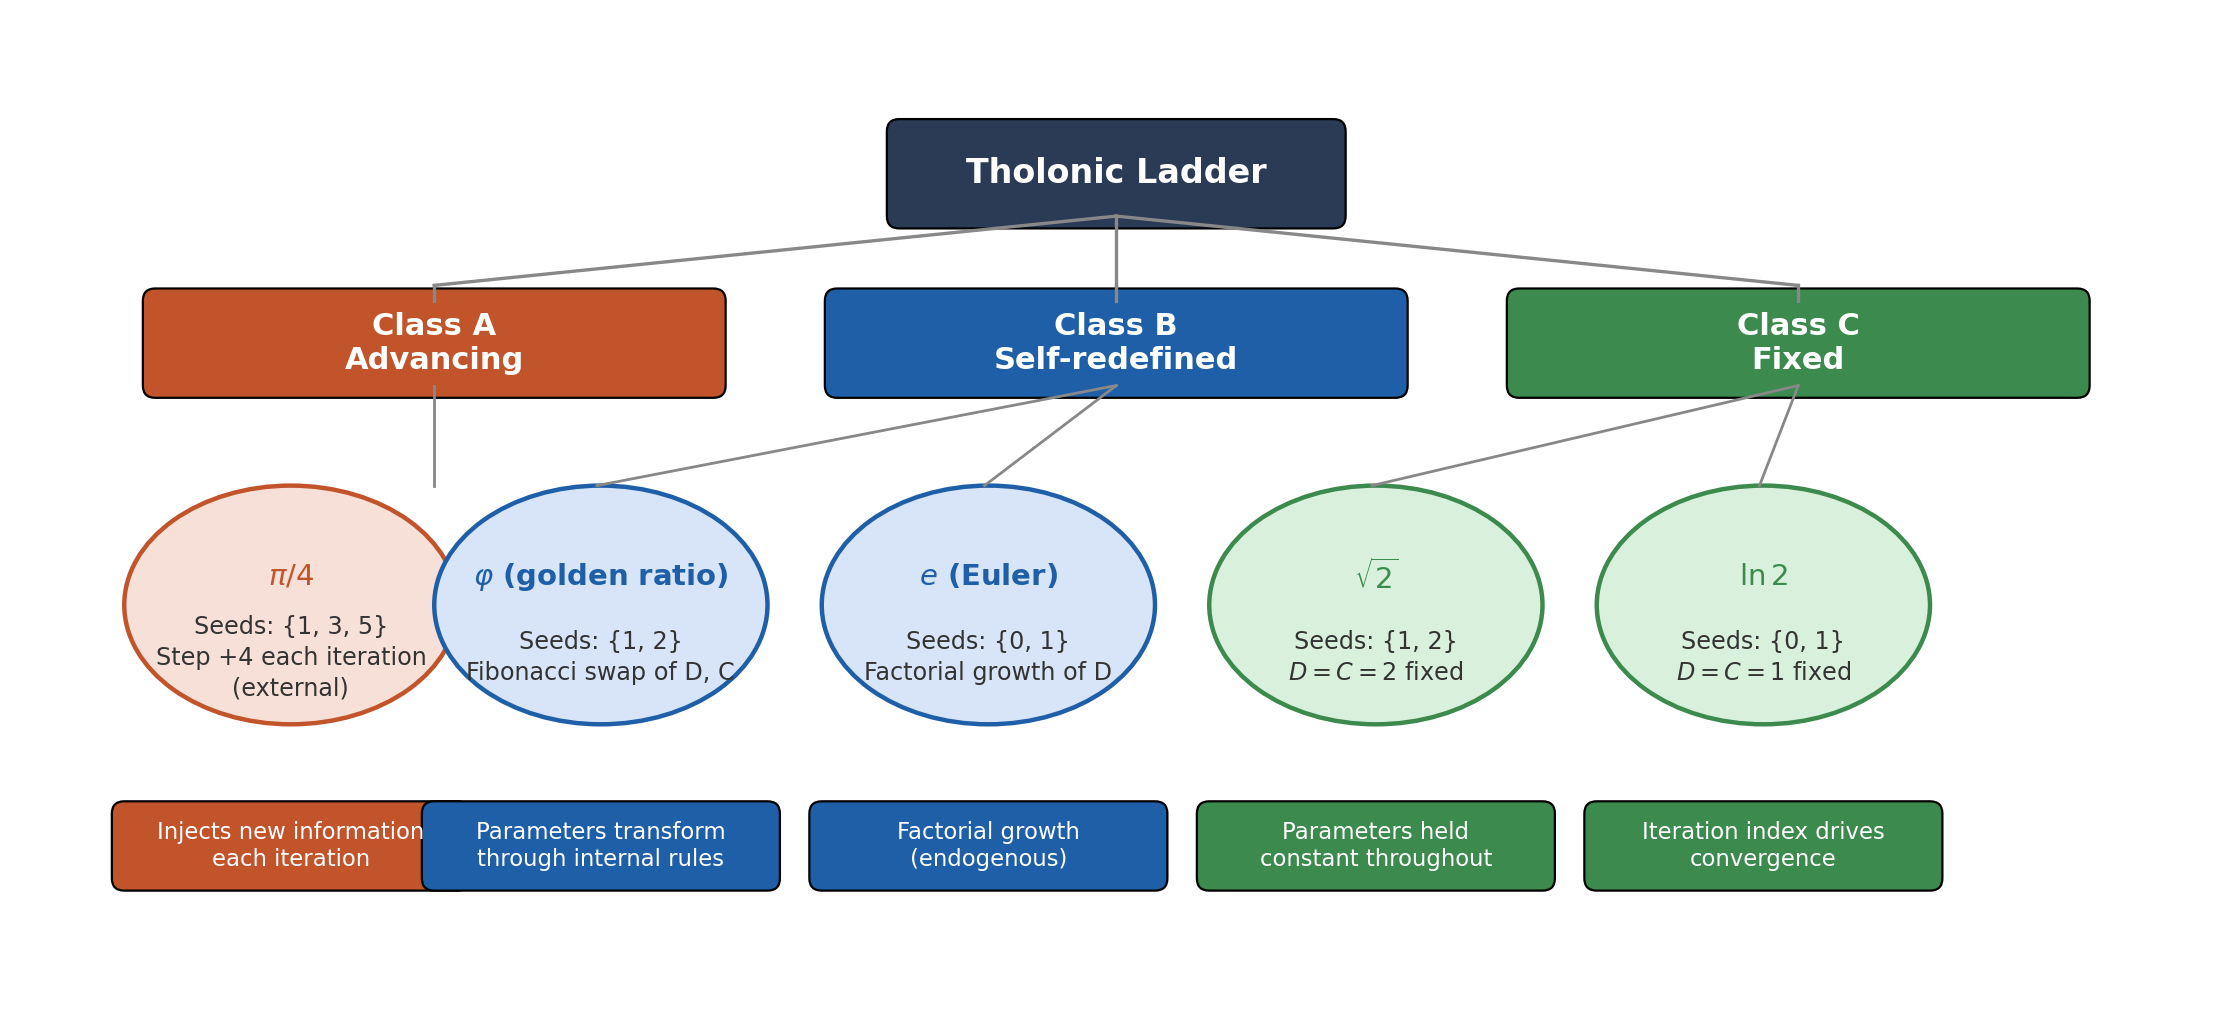
\includegraphics[width=\linewidth,keepaspectratio]{figures/1_traversal-classes}
  \caption{Classification of the five tholonic ladder branches by traversal type.
    Class~A (red) injects new information each step via an external increment.
    Class~B (blue) evolves parameters by an internal rule.
    Class~C (green) holds all parameters fixed; convergence is driven by the update map
    alone, with the iteration index entering $f$ directly in the $\ln 2$ branch.}
  \label{fig:traversal-classes}
\end{figure}

\section{Branch specification and convergence proofs}\label{sec:branches}

{\renewcommand{\arraystretch}{2.6}
\begin{table}[ht]
\centering
\caption{Complete branch specification.}\label{tab:branches}
\begin{tabular}{lccc>{\centering\arraybackslash}p{4cm}lc}
\toprule
Limit & $N_0$ & $D_0$ & $C_0$ & $N_{k+1}$ & Traversal rule & Class \\
\midrule
$\pi/4$    & 1 & 3 & 5
  & $\displaystyle N - \dfrac{1}{D} + \dfrac{1}{C}$
  & $D \leftarrow D+4,\quad C \leftarrow C+4$ & A \\
$\varphi$  & 1 & 1 & 2
  & $\displaystyle N_0 + \dfrac{D}{C}$
  & $D \leftarrow C,\quad C \leftarrow C + D$ & B \\
$e$        & 0 & 1 & 1
  & $\displaystyle N + \dfrac{D}{C}$
  & $C \leftarrow C \cdot \max(k,1)$ & B \\
$\sqrt{2}$ & 1 & 2 & 2
  & $\displaystyle\dfrac{N + D/N}{C}$
  & $D,\,C$ fixed & C \\
$\ln 2$    & 0 & 1 & 1
  & $\displaystyle N + (-1)^k \dfrac{D}{k + C}$
  & $D,\,C$ fixed & C \\
\bottomrule
\end{tabular}
\end{table}}

In every branch $D$ plays the bounding/constraining role and $C$ the
integrating/synthesizing role, despite the operations differing.
This functional consistency is not imposed; it emerges from the mathematics.

\subsection{The \texorpdfstring{$\pi/4$}{pi/4} branch}\label{subsec:pi4}

\begin{proposition}\label{prop:pi4}
With $(N_0, D_0, C_0) = (1, 3, 5)$ and step $\Delta = 4$,
\[
  N_\infty = 1 + \sum_{n=1}^{\infty}\!\left(\frac{1}{4n+1} - \frac{1}{4n-1}\right)
           = 1 + \sum_{n=1}^{\infty}\frac{-2}{16n^2-1} = \frac{\pi}{4}.
\]
\end{proposition}

\begin{proof}
At iteration $n \geq 1$, $D_n = 4n-1$ and $C_n = 4n+1$. The update adds
$-1/(4n-1) + 1/(4n+1) = -2/(16n^2-1)$. Starting from $N_0 = 1$,
the accumulated sum is a grouping of consecutive Leibniz pairs. By the alternating series
theorem applied to $\sum_{k=0}^\infty (-1)^k/(2k+1)$, the grouped sum converges to $\pi/4$
\cite{Kno56}.
\end{proof}

\begin{remark}[Primitive invariant]
The recurrence targets $\pi/4$ directly; $\pi = 4(\pi/4)$ is a geometric normalization.
We treat $\pi/4$ as the \emph{primitive invariant} of this branch.
\end{remark}

\begin{corollary}[Perfect-square form]\label{cor:perfect-square-form}
Multiplying both sides of Proposition~\ref{prop:pi4} by $8$:
\[
  \pi = \sum_{n=1}^{\infty} \frac{8}{16n^2 - 1},
\]
expressing $\pi$ in terms of perfect squares offset by unity. See also
Proposition~\ref{prop:perfect-squares}.
\end{corollary}

\textbf{Functional roles.} $D_k$ subtracts from $N_k$ (constraining); $C_k$ adds
(contributing). Both advance in lockstep, driven by external step $\Delta = 4$.

\begin{figure}[ht]
  \centering
  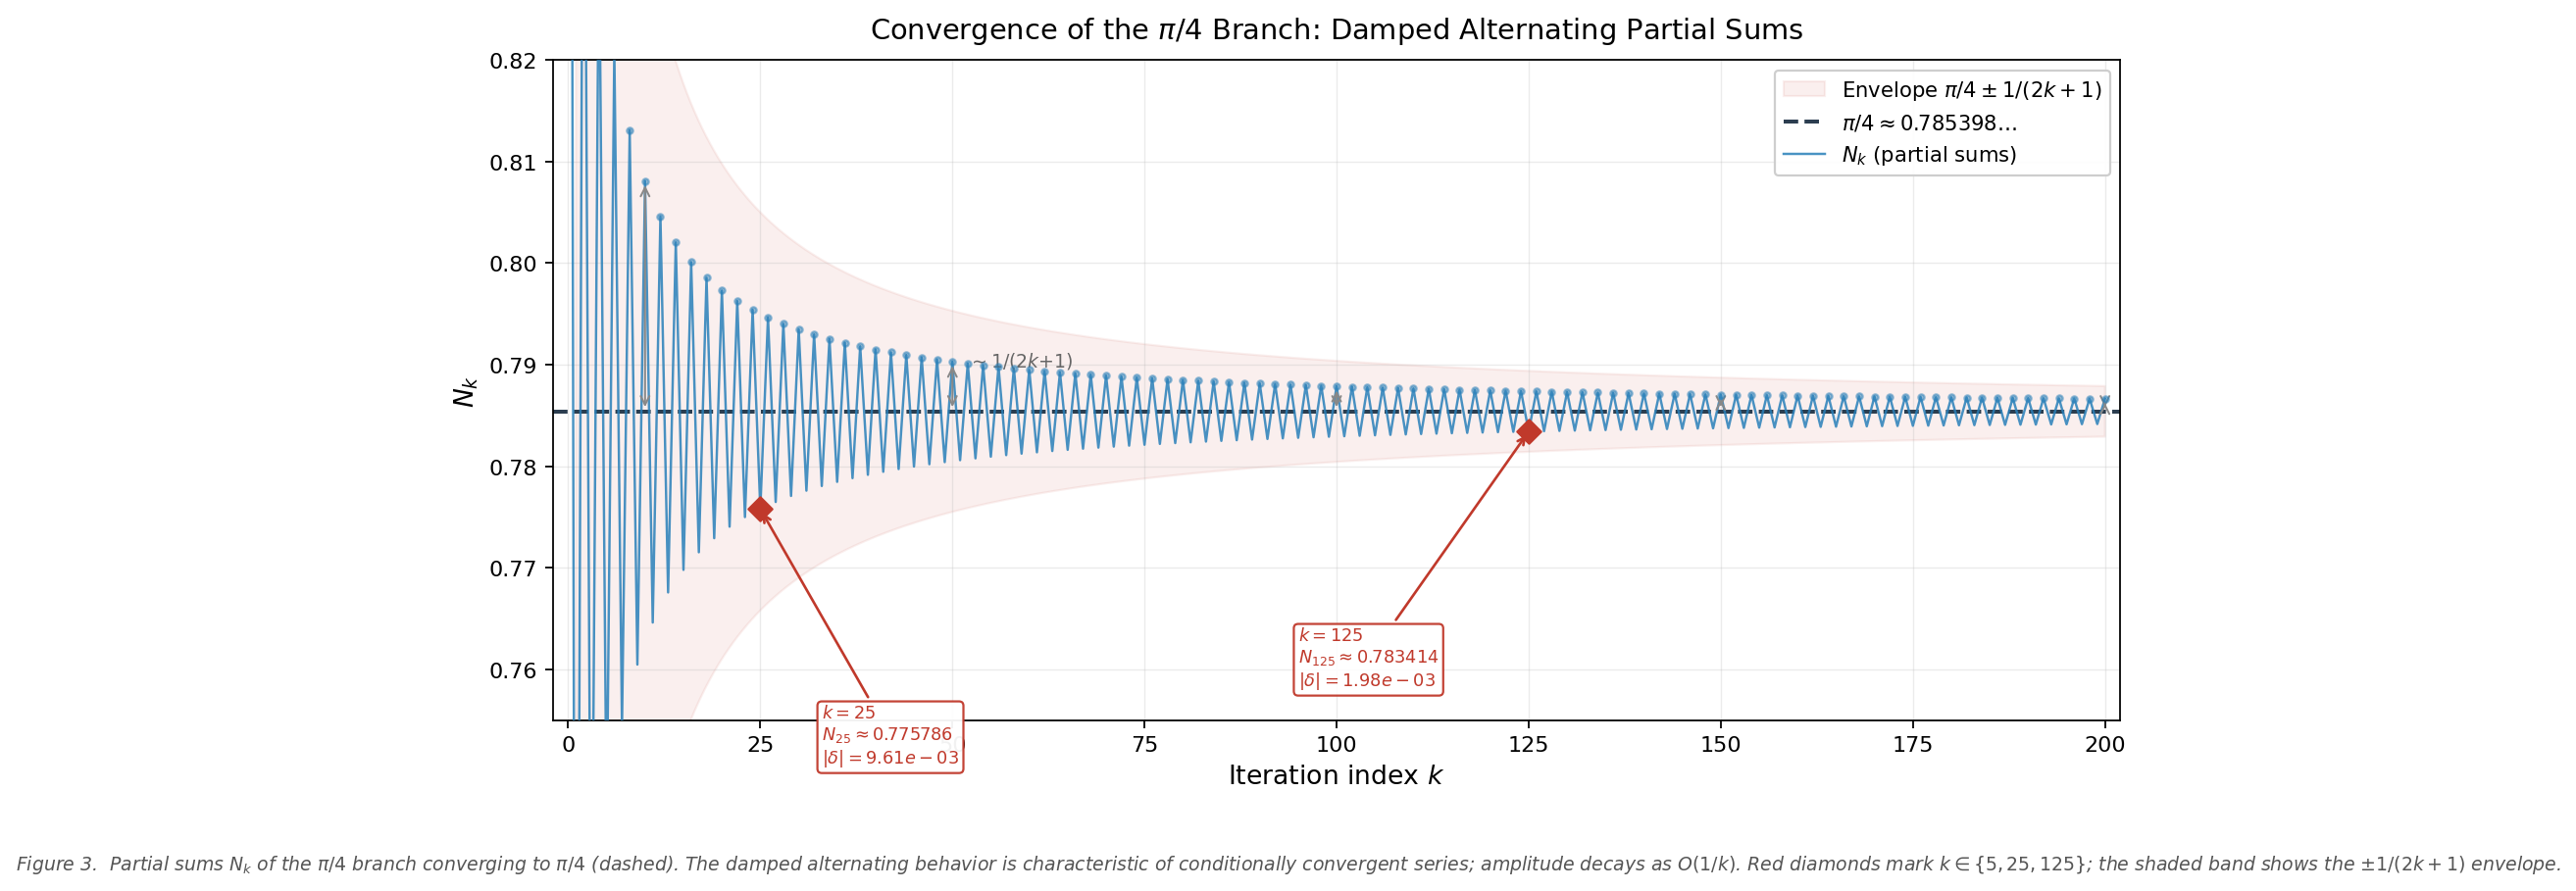
\includegraphics[width=\linewidth,keepaspectratio]{figures/1_pi4-convergence}
  \caption{Partial sums $N_k$ of the $\pi/4$ branch converging to $\pi/4$ (dashed).
    Amplitude decays as $O(1/k)$. Red diamonds mark $k \in \{5, 25, 125\}$;
    the shaded band shows the $\pm 1/(2k+1)$ envelope.}
  \label{fig:pi4-convergence}
\end{figure}

\subsection{The \texorpdfstring{$\varphi$}{phi} branch}\label{subsec:phi}

\begin{proposition}\label{prop:phi}
With $(N_0, D_0, C_0) = (1, 1, 2)$, update $N_{k+1} = N_0 + D_k/C_k$, and the Fibonacci
traversal $D \leftarrow C$, $C \leftarrow C + D$, the limit is
$N_\infty = \varphi = (1+\sqrt{5})/2$.
\end{proposition}
\begin{proof}
With seeds $(D_0, C_0) = (1, 2) = (F_2, F_3)$, the traversal maintains
$(D_k, C_k) = (F_{k+2}, F_{k+3})$, consecutive Fibonacci numbers. Ratios of consecutive
Fibonacci numbers converge: $F_{k+2}/F_{k+3} \to 1/\varphi$ \cite{HW79,Kos01}, with error
contracting geometrically by the factor $\varphi^{-2} \approx 0.382$ per step (Binet's
formula). Hence $N_{k+1} = 1 + F_{k+2}/F_{k+3} \to 1 + 1/\varphi = \varphi$, by the
defining identity $\varphi = 1 + 1/\varphi$.
\end{proof}
\textbf{Functional roles.} $D$ is the smaller (prior) Fibonacci term; the boundary.
$C$ is the larger accumulated term; the integration of the two most recent generations.
The update consumes the ratio $D/C$ directly, so the Fibonacci traversal is the engine
of convergence, not an accessory to it.

\subsection{The \texorpdfstring{$\sqrt{2}$}{sqrt(2)} branch}\label{subsec:sqrt2}

\begin{proposition}\label{prop:sqrt2}
With $(N_0, D_0, C_0) = (1, 2, 2)$ and fixed parameters, $N_\infty = \sqrt{2}$, with quadratic convergence.
\end{proposition}
\begin{proof}
The update $N_{k+1} = (N_k + 2/N_k)/2$ is the Newton--Babylonian method for $x^2 = 2$
\cite{Hea21,BF15}. Let $g(x) = (x + 2/x)/2$. Then $g(\sqrt{2}) = \sqrt{2}$ and
$g^{\prime}(\sqrt{2}) = (1 - 2/x^2)/2\big|_{x=\sqrt{2}} = 0$, confirming quadratic convergence.
\end{proof}
\textbf{Functional roles.} $D = 2$ is the target; the defining constraint. $C = 2$ is the
averaging divisor. Though $D = C$ numerically, their roles are distinct.

\subsection{The \texorpdfstring{$e$}{e} branch}\label{subsec:e}

\begin{proposition}\label{prop:e}
With $(N_0, D_0, C_0) = (0, 1, 1)$ and $C_k = k!$, $N_\infty = e$.
\end{proposition}
\begin{proof}
The update $N_{k+1} = N_k + 1/k!$ accumulates $\sum_{k=0}^{K} 1/k!$, converging to $e$ \cite{Rud76}.
\end{proof}
\textbf{Functional roles.} $D = 1$ is the fixed numerator; the unchanging boundary.
$C$ starts at~$1$ but grows as a factorial: the expanding denominator.
\begin{remark}[Offset variant]
When initialized with $N_0 = 2$, the branch converges to $e + 2$, confirming the offset
$= N_0$ (Proposition~\ref{prop:offset}).
\end{remark}

\subsection{The \texorpdfstring{$\ln 2$}{ln 2} branch}\label{subsec:ln2}

\begin{proposition}\label{prop:ln2}
With $(N_0, D_0, C_0) = (0, 1, 1)$ and fixed parameters, $N_\infty = \ln 2$.
\end{proposition}
\begin{proof}
The update accumulates $(-1)^k/(k+1)$ starting at $k = 0$, giving
$\sum_{k=0}^\infty (-1)^k/(k+1) = \ln 2$ \cite{Kno56}.
\end{proof}
\textbf{Functional roles.} $D = 1$ is the fixed numerator; $C = 1$ is the integration base.
They are numerically identical but structurally distinct: one limits, one integrates.
\begin{remark}[Offset variant]
When $N_0 = 1/2$, the branch converges to $\ln 2 + 1/2$. The offset equals $N_0$ exactly,
as it must: the update is pure accumulation, so the seed enters the limit additively
(Proposition~\ref{prop:offset}).
\end{remark}

\section{Structural properties}\label{sec:structural}

\begin{proposition}[Seed partition]\label{prop:seed-partition}
Among the five branches, the $\pi/4$ branch is the unique branch with three numerically
distinct seeds; its seed set is $\{1, 3, 5\}$. The remaining four branches have seeds
drawn from $\{0, 1, 2\}$.
\end{proposition}
\begin{table}[ht]
\centering\caption{Seed partition across the five branches.}\label{tab:seed-partition}
\begin{tabular}{lccl}\toprule
Branch & Seeds & Distinct values & Seed set \\\midrule
$\pi/4$    & $(1,3,5)$ & 3 & $\{1,3,5\}$ \\
$\varphi$  & $(1,1,2)$ & 2 & $\{1,2\}$ \\
$e$        & $(0,1,1)$ & 2 & $\{0,1\}$ \\
$\sqrt{2}$ & $(1,2,2)$ & 2 & $\{1,2\}$ \\
$\ln 2$    & $(0,1,1)$ & 2 & $\{0,1\}$ \\\bottomrule
\end{tabular}\end{table}
The value~$1$ appears 10 out of 15 times. Only $\pi/4$ demands the richer seed set
$\{1, 3, 5\}$ and external parameter injection.
\begin{remark}[Seeds and primality]
The seeds $1, 3, 5$ are the first three odd integers $\geq 1$. Whether $1$ is treated
as ``prime'' does not affect the convergence proof; it is the generative unit from
which the triadic recursion begins.
\end{remark}

\begin{proposition}[Diagonal invariance]\label{prop:diagonal}
For the Class~A recurrence with $D_k = C_k$ for all $k$, the partial sums telescope
to zero and $N_\infty = N_0$. Non-triviality requires $D \neq C$.
\end{proposition}
\begin{proof}
At each step, $-1/D_k + 1/C_k = 0$ when $D_k = C_k$. The running total is unchanged.
\end{proof}

\begin{proposition}[Swap symmetry]\label{prop:swap}
For the Class~A recurrence with fixed $N_0$, let $N_\infty(D_0, C_0)$ denote the limit.
Then $N_\infty(D_0, C_0) + N_\infty(C_0, D_0) = 2\,N_0$.
\end{proposition}
\begin{proof}
Swapping $D \leftrightarrow C$ negates the signed contribution $-1/D_k + 1/C_k$ at
every step, so the two accumulated partial sums are antisymmetric around $N_0$.
\end{proof}
\begin{figure}[ht]
  \centering
  \includegraphics[width=\linewidth,keepaspectratio]{figures/1_swap-symmetry}
  \caption{Swap symmetry (Proposition~\ref{prop:swap}): runs $(3,5)$ and $(5,3)$ mirror
    around $N_0=1$. Run~A decreases to $\pi/4$; Run~B increases to $2-\pi/4$.
    Equal brackets confirm $N_A(k)+N_B(k)=2$ at each step.}
  \label{fig:swap-symmetry}
\end{figure}

\begin{proposition}[Perfect-square denominators]\label{prop:perfect-squares}
In the $\pi/4$ branch, $D_n \cdot C_n = (4n-1)(4n+1) = 16n^2 - 1$ for $n \geq 1$.
This yields
\[
  \pi = \sum_{n=1}^{\infty} \frac{8}{16n^2 - 1}.
\]
\end{proposition}
\begin{proof}
With $D_n = 4n-1$ and $C_n = 4n+1$, the product is $16n^2-1$. The identity for $\pi$
follows from Proposition~\ref{prop:pi4} by algebraic rearrangement.
\end{proof}
\begin{table}[ht]
\centering\caption{Denominator products.}\label{tab:perfect-squares}
\begin{tabular}{ccccc}\toprule
$n$ & $D_n$ & $C_n$ & $D_n \cdot C_n$ & Perfect-square form \\\midrule
1 &  3 &  5 &  15 & $16(1)^2 - 1$ \\
2 &  7 &  9 &  63 & $16(2)^2 - 1$ \\
3 & 11 & 13 & 143 & $16(3)^2 - 1$ \\\bottomrule
\end{tabular}\end{table}
\begin{figure}[ht]
  \centering
  \includegraphics[width=\linewidth,keepaspectratio]{figures/1_perfect-squares}
  \caption{The products $D_n \cdot C_n = 16n^2-1$ at scales $K = 10, 100, 1000$.
    Each scale reproduces the same parabolic shape. Dotted red: reference parabola $16n^2$.}
  \label{fig:perfect-squares}
\end{figure}

\begin{proposition}[Offset consistency, translation equivariance]\label{prop:offset}
Let a branch have a pure-accumulation update $N_{k+1} = N_k + t_k$, where the term $t_k$
depends only on $(D_k, C_k, k)$ and not on $N_k$ (the $e$ and $\ln 2$ branches). Then the
limit is translation-equivariant in the seed:
\[
  N_\infty(N_0) = N_0 + N_\infty(0),
\]
so the affine offset of $N_\infty$ from the target constant equals $N_0$ exactly.
\end{proposition}
\begin{proof}
By induction, $N_K = N_0 + \sum_{k=0}^{K-1} t_k$, and the sum is independent of $N_0$.
Letting $K \to \infty$ gives the identity.
\end{proof}
\begin{table}[ht]
\centering\caption{Offset behavior.}\label{tab:offset}
\begin{tabular}{lccc}\toprule
Branch & Variant $N_0$ & $N_\infty$ & Offset \\\midrule
$e$     & $2$   & $e + 2$       & $+2 = N_0$ \\
$\ln 2$ & $1/2$ & $\ln 2 + 1/2$ & $+1/2 = N_0$ \\\bottomrule
\end{tabular}\end{table}
In both cases the offset is the initial baseline. In the canonical forms (Table~\ref{tab:branches})
with $N_0 = 0$, both converge directly to their targets.

\begin{proposition}[Parametric families]\label{prop:parametric}
Two branches embed in one-parameter families with the same traversal class and role structure:
\emph{(i)}~replacing $D = 2$ by $D = a > 0$ in the $\sqrt{2}$ branch yields
$N_\infty = \sqrt{a}$, with quadratic convergence, for every $a$;
\emph{(ii)}~replacing the additive base $N_0 = 1$ by $m \in \mathbb{N}$ in the $\varphi$
branch, with the generalized traversal $D \leftarrow C$, $C \leftarrow mC + D$, yields the
metallic means $N_\infty = \sigma_m = (m + \sqrt{m^2 + 4})/2$; the case $m = 1$ recovers $\varphi$.
\end{proposition}
\begin{proof}
\emph{(i)} The update $N_{k+1} = (N_k + a/N_k)/C$ with $C = 2$ is Newton's method for
$x^2 = a$ \cite{BF15}; the argument of Proposition~\ref{prop:sqrt2} applies verbatim, with
$g^{\prime}(\sqrt{a}) = 0$ giving quadratic convergence.
\emph{(ii)} The traversal maintains consecutive terms of the generalized Fibonacci
recurrence $G_{k+1} = m G_k + G_{k-1}$, whose consecutive ratios converge (for any
positive seeds, since $\sigma_m$ is the dominant root) to the positive root of
$x^2 = mx + 1$: thus $D_k/C_k \to 1/\sigma_m$, and
$N_{k+1} = m + D_k/C_k \to m + 1/\sigma_m = \sigma_m$ by the defining identity
$\sigma_m = m + 1/\sigma_m$.
\end{proof}
These deformations show that the documented branches are distinguished points inside
parametric families rather than isolated curiosities, and they make precise why the
local-isolation reformulation of Conjecture~\ref{conj:finite} is the natural one: within
a family, varying the parameter moves the limit continuously through other algebraic
targets, so uniqueness claims must be made relative to fixed parameters.

\section{Convergence}\label{sec:convergence}
\begin{table}[ht]
\centering\caption{Numerical convergence at $K = 10^5$ iterations.}\label{tab:convergence}
\begin{tabular}{lllll}\toprule
Branch & $N_K$ (computed) & Target & Residual & Rate \\\midrule
$\pi/4$    & $0.785\,399\,4\ldots$ & $0.785\,398\,2\ldots$ & $1.2 \times 10^{-6}$ & $O(1/K)$ \\
$\varphi$  & $1.618\,033\,9\ldots$ & $1.618\,033\,9\ldots$ & $< 10^{-15}$ & linear, rate $\varphi^{-2}$ \\
$e$        & $2.718\,281\,8\ldots$ & $2.718\,281\,8\ldots$ & $< 10^{-15}$ & $O(1/K!)$ \\
$\sqrt{2}$ & $1.414\,213\,6\ldots$ & $1.414\,213\,6\ldots$ & $< 10^{-15}$ & quadratic \\
$\ln 2$    & $0.693\,142\,2\ldots$ & $0.693\,147\,2\ldots$ & $5.0 \times 10^{-6}$ & $O(1/K)$ \\\bottomrule
\end{tabular}\end{table}
The slow convergence of $\pi/4$ and $\ln 2$ is intrinsic to their alternating-series structure.
The three remaining branches converge to machine precision well within $10^5$ iterations.
Series-acceleration methods (Euler, van~Wijngaarden, Levin) would reduce residuals for
the two slow branches but are not required by the framework.

\textbf{Explicit error bounds.} For the two alternating branches the alternating series
theorem supplies a priori envelopes: after $k$ iterations,
$|N_k - \pi/4| \leq 1/(4k+3)$ (the first omitted Leibniz term) and
$|N_k - \ln 2| \leq 1/(k+1)$. At $K = 10^5$ these give $2.5 \times 10^{-6}$ and $10^{-5}$,
consistent with the observed residuals $1.2 \times 10^{-6}$ and $5.0 \times 10^{-6}$
(roughly half the envelope, as expected for an alternating tail). For $\sqrt{2}$, Newton's
method gives the exact one-step relation
$|N_{k+1} - \sqrt{2}| = |N_k - \sqrt{2}|^2 / (2N_k)$; for $\varphi$, the error contracts
geometrically by the factor $\varphi^{-2} \approx 0.382$ per step.
\begin{figure}[ht]
  \centering
  \includegraphics[width=\linewidth,keepaspectratio]{figures/1_convergence-comparison}
  \caption{Convergence of all five branches: $\log_{10}|N_k - N_\infty|$ vs.\ $k$ at
    $K = 10^5$ iterations. Class~B branches reach machine precision within tens of steps;
    Class~C Newton--Babylonian ($\sqrt{2}$) converges quadratically by $k \approx 6$.
    Class~A ($\pi/4$) and Class~C ($\ln 2$) decay as $O(1/k)$.}
  \label{fig:convergence-comparison}
\end{figure}

\textbf{Convergence and traversal class.} The two slowest branches are Class~A ($\pi/4$)
and one Class~C branch ($\ln 2$). The fastest are Class~B ($e$, super-exponential;
$\varphi$, linear with geometric ratio $\varphi^{-2} \approx 0.382$) and the other
Class~C branch ($\sqrt{2}$, quadratic).

\section{Open problems}\label{sec:open}
The structural results of \S\,\ref{sec:structural} are proved. The following questions
remain open; positive resolutions would move the framework from taxonomy to theorem.
\begin{conjecture}[Uniqueness of the $\pi/4$ seed]\label{conj:uniqueness}
The seed triple $(1, 3, 5)$ is the unique Class~A admissible seed with $D_0 < C_0$,
$C_0 - D_0 = 2$, $D_0$ and $C_0$ consecutive in the $\{4n-1\}$ and $\{4n+1\}$ sequences,
that yields $N_\infty = \pi/4$ under step size $\Delta = 4$.
\end{conjecture}
\begin{conjecture}[Exclusion from the $\{0,1,2\}$ lattice]\label{conj:exclusion}
No triple $(N_0, D_0, C_0) \in \{0,1,2\}^3$ with any Class~B or Class~C traversal rule
yields $N_\infty = \pi/4$. That is, $\pi/4$ is genuinely inaccessible from the primitive
seed lattice.
\end{conjecture}
\begin{conjecture}[Finite classification]\label{conj:finite}
There exists a finite rule set $\mathcal{R}$ such that the only convergent branches with
limits in $\{\pi/4, \varphi, e, \sqrt{2}, \ln 2\}$ are exactly the five documented here.
\end{conjecture}
If Conjecture~\ref{conj:finite} fails, the appropriate reformulation is: show the five branches
are \emph{locally isolated} within the admissible space.
\begin{conjecture}[Non-circularity of the $\pi/4$ grouping]\label{conj:noncircularity}
The pairing $N_{k+1} = N_k - 1/D_k + 1/C_k$ with Class~A advancement can be derived from
constraints \emph{(a)}~$f$ is rational of degree $\leq 1$ in $D^{-1}$ and $C^{-1}$,
\emph{(b)}~$D$ and $C$ carry opposite signs, and \emph{(c)}~step $\Delta$ is derived from
the Instantiation axis, without assuming $\pi$ as input.
\end{conjecture}
Conjecture~\ref{conj:noncircularity} is the key independence question. Establishing it would
show that the $\pi/4$ grouping is structurally forced, not chosen post hoc.

\section{Related work}\label{sec:related}
\textbf{Series rearrangements.} The Leibniz series is conditionally convergent, so
rearrangements can alter its sum \cite{Kno56}. The $\pi/4$ branch uses \emph{grouped}
(paired) rearrangement, not a sign-pattern reordering, so its limit is standard.
\textbf{Continued fractions and metallic means.} The golden ratio is the simplest nontrivial
continued fraction, $\varphi = [1;1,1,1,\ldots]$, and the worst-approximable irrational
\cite{HW79}. The $\varphi$ branch recovers this via Fibonacci recursion without competing
with continued-fraction theory \cite{Kos01}; the metallic means extend the same template
parametrically (Proposition~\ref{prop:parametric}).
\textbf{Newton--Babylonian method.} The $\sqrt{2}$ branch is the classical Heron iteration
for $x^2 = 2$ \cite{Hea21,BF15}. The tholonic framing adds role interpretation without
altering the proof or convergence order.
\textbf{Classical series identities.} Standard analysis establishes $\sum_{k=0}^\infty 1/k! = e$
\cite{Rud76} and $\sum_{k=1}^\infty (-1)^{k+1}/k = \ln 2$ \cite{Kno56}. The ladder presents
these as Class~B and~C branches in a unified format.
\textbf{Structural unification.} We are unaware of a framework that identifies all five of
$\pi/4$, $\varphi$, $e$, $\sqrt{2}$, $\ln 2$ as branches of a common three-variable
recurrence with consistent role assignments.
\textbf{Leibniz and binary structure.} Leibniz developed binary arithmetic simultaneously
with the $\pi/4$ series and drew connections to the I~Ching \cite{Lei03,Swe03}.

\section{Discussion}\label{sec:discussion}
\textbf{Organizational vs.\ predictive claims.} The ladder framework as proved is
\emph{organizational}: a unified format from which five known limits descend. The path
from organizational to predictive runs through the Conjectures of \S\,\ref{sec:open}.
\textbf{Post hoc flexibility risk.} The standard referee objection is: ``you chose seeds
and rules after knowing the targets.'' The structural theorems partially defuse this.
Diagonal invariance and swap symmetry are consequences of the Class~A form independent of
any targeted limit. The seed partition (Proposition~\ref{prop:seed-partition}) is a sharp
combinatorial observation: a framework tuned post hoc would not automatically produce a
clean $\{1,3,5\}$ vs.\ $\{0,1,2\}$ partition.

The remaining vulnerability is Conjecture~\ref{conj:noncircularity}. Until non-circularity
is established for the $\pi/4$ grouping, one cannot rule out that it is one among infinitely
many valid Leibniz rearrangements that happen to fit the Class~A format.

\textbf{Convergence rates as a structural signal.} The two $O(1/k)$ branches are Class~A
($\pi/4$) and a Class~C branch ($\ln 2$); the other three reach machine precision within
tens of iterations ($e$ super-exponentially, $\sqrt{2}$ quadratically, $\varphi$ linearly
at geometric ratio $\varphi^{-2}$). The per-step ordering places Class~C $\sqrt{2}$
(quadratic) above Class~B $\varphi$ (linear), so the correlation between traversal class
and convergence order is imperfect; characterizing exactly when class predicts rate is an
open regularity.

\textbf{The infinite landscape.} The five branches are recognizable loci in an infinite
space of admissible seed--traversal combinations. Proposition~\ref{prop:parametric}
exhibits two parametric families explicitly: the square roots $\sqrt{a}$ and the metallic
means $\sigma_m$. The scientific question is which of the infinite admissible paths yield
limits of independent mathematical significance, and whether that set is finite and
well-characterized.

\section{Conclusion}\label{sec:conclusion}
We have presented a three-variable recurrence family $(N, D, C)$, the tholonic ladder,
with five branches converging to $\pi/4$, $\varphi$, $e$, $\sqrt{2}$, and $\ln 2$.
The limits are classical; the contribution lies in the structural theorems: a seed partition
cleanly separating the $\pi/4$ branch, diagonal invariance and swap symmetry for the
Class~A template, a perfect-square denominator identity linking $\pi$ to the step structure,
an offset-consistency law for shifted initializations, and two parametric families
(square roots and metallic means) embedding the $\sqrt{2}$ and $\varphi$ branches.

The central claim (\textbf{same recursive triadic geometry, different traversal dynamics,
different limits}) is supported by these proved contrasts. The open work, stated as four
numbered conjectures, concerns whether the seed assignments and traversal rules are forced
by a small set of axioms (predictive framework) or represent a human-chosen sample
(organizational taxonomy). The structural evidence points toward the former; the proofs
are not yet in hand.

\appendix
\section{Reference implementation}\label{app:impl}
The following Python code implements all five branches. No bare numeric literals appear
inside any recursion loop.

\begin{lstlisting}[language=Python,caption={Reference implementation.},label={lst:impl}]
#!/usr/bin/env python3

def _compute_pi_over_4(max_iter, istep=2):
    N, D, C = 1.0, 3.0, 5.0
    d_step = istep ** 2;  c_step = istep * 2
    for _ in range(max_iter):
        N = N - (1.0 / D) + (1.0 / C)
        D += d_step;  C += c_step
    return N

def _compute_phi(max_iter):
    N = 1.0
    D, C = 1, 2   # exact integer Fibonacci terms (floats overflow near k = 1476)
    base = N
    for _ in range(max_iter):
        N = base + (D / C);  D, C = C, (C + D)
    return N

def _compute_e(max_iter):
    N, D, C = 0.0, 1.0, 1.0
    for count in range(max_iter):
        N = N + (D / C);  C *= count + 1 if count > 0 else 1
    return N

def _compute_sqrt2(max_iter):
    N, D, C = 1.0, 2.0, 2.0
    for _ in range(max_iter):
        N = (N + (D / N)) / C
    return N

def _compute_ln2(max_iter):
    N, D, C = 0.0, 1.0, 1.0
    for count in range(max_iter):
        term = D / (count + C)
        N = N + term if count % 2 == 0 else N - term
    return N

\end{lstlisting}

\textbf{Output at $10^5$ iterations:}
\begin{verbatim}
pi/4   = 0.7853994133911905
phi    = 1.618033988749895
e      = 2.7182818284590455
sqrt2  = 1.414213562373095
ln2    = 0.6931421805849816
\end{verbatim}

\section{Summary table with convergence rates}\label{app:summary}
\begin{table}[ht]
\centering\caption{Summary of all five branches.}\label{tab:summary}
\begin{tabular}{llllll}\toprule
Target & $(N_0,D_0,C_0)$ & Seed set & Class & Classical mechanism & Rate \\\midrule
$\pi/4$    & $(1,3,5)$ & $\{1,3,5\}$ & A & Leibniz paired grouping  & $O(1/K)$ \\
$\varphi$  & $(1,1,2)$ & $\{1,2\}$   & B & Fibonacci ratio convergence & linear, rate $\varphi^{-2}$ \\
$e$        & $(0,1,1)$ & $\{0,1\}$   & B & $\sum_{k=0}^\infty 1/k!$ & $O(1/K!)$ \\
$\sqrt{2}$ & $(1,2,2)$ & $\{1,2\}$   & C & Newton--Babylonian       & quadratic \\
$\ln 2$    & $(0,1,1)$ & $\{0,1\}$   & C & alternating harmonic     & $O(1/K)$ \\\bottomrule
\end{tabular}\end{table}
Offset behavior: see Proposition~\ref{prop:offset}.

\bibliographystyle{plainnat}
\bibliography{refs}
\end{document}
